\question \textbf{Bet On It} \\*
Smith is in jail and has 3 dollars; he can get out on bail if he has 
8 dollars. A guard agrees to make a series of bets with him. If Smith 
bets A dollars, he wins A dollars with probability 0.4 and loses A 
dollars with probability 0.6.
\begin{enumerate}[label=\alph*)]
\item
Find the probability that he wins 8 dollars before losing all of his 
money if he bets 1 dollar each time. 
\begin{solution}[8cm]
The Markov chain $(X_n, n = 0, 1, \dots)$ representing the evolution 
of Smith's money has diagram

\begin{center}
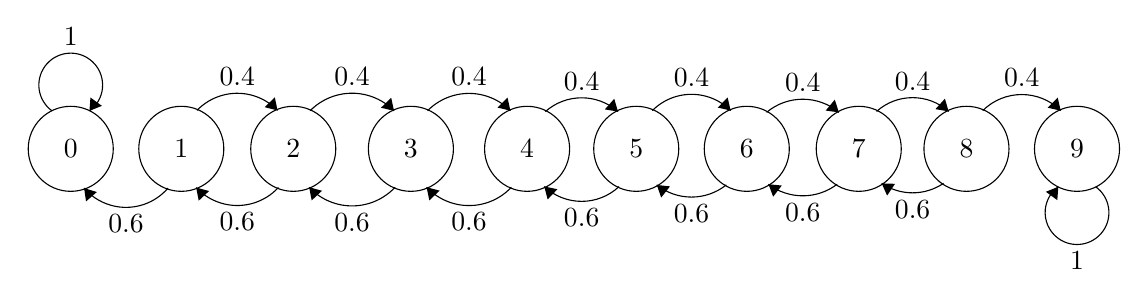
\begin{tikzpicture}[scale=0.18]
\tikzstyle{every node}+=[inner sep=0pt]
\draw [black] (7.9,-33.6) circle (3);
\draw (7.9,-33.6) node {$0$};
\draw [black] (15.7,-33.6) circle (3);
\draw (15.7,-33.6) node {$1$};
\draw [black] (23.6,-33.6) circle (3);
\draw (23.6,-33.6) node {$2$};
\draw [black] (31.9,-33.6) circle (3);
\draw (31.9,-33.6) node {$3$};
\draw [black] (40.1,-33.6) circle (3);
\draw (40.1,-33.6) node {$4$};
\draw [black] (47.8,-33.6) circle (3);
\draw (47.8,-33.6) node {$5$};
\draw [black] (55.6,-33.6) circle (3);
\draw (55.6,-33.6) node {$6$};
\draw [black] (63.5,-33.6) circle (3);
\draw (63.5,-33.6) node {$7$};
\draw [black] (71.1,-33.6) circle (3);
\draw (71.1,-33.6) node {$8$};
\draw [black] (78.9,-33.6) circle (3);
\draw (78.9,-33.6) node {$9$};
\draw [black] (6.577,-30.92) arc (234:-54:2.25);
\draw (7.9,-26.35) node [above] {$1$};
\fill [black] (9.22,-30.92) -- (10.1,-30.57) -- (9.29,-29.98);
\draw [black] (14.762,-36.372) arc (-40.68932:-139.31068:3.907);
\fill [black] (8.84,-36.37) -- (8.98,-37.31) -- (9.74,-36.65);
\draw (11.8,-38.23) node [below] {$0.6$};
\draw [black] (22.549,-36.333) arc (-42.79165:-137.20835:3.95);
\fill [black] (16.75,-36.33) -- (16.93,-37.26) -- (17.66,-36.58);
\draw (19.65,-38.1) node [below] {$0.6$};
\draw [black] (16.806,-30.889) arc (136.04575:43.95425:3.95);
\fill [black] (22.49,-30.89) -- (22.3,-29.97) -- (21.58,-30.66);
\draw (19.65,-29.18) node [above] {$0.4$};
\draw [black] (30.782,-36.314) arc (-43.09717:-136.90283:4.152);
\fill [black] (24.72,-36.31) -- (24.9,-37.24) -- (25.63,-36.56);
\draw (27.75,-38.13) node [below] {$0.6$};
\draw [black] (24.788,-30.916) arc (135.44555:44.55445:4.156);
\fill [black] (30.71,-30.92) -- (30.51,-30) -- (29.79,-30.7);
\draw (27.75,-29.18) node [above] {$0.4$};
\draw [black] (38.987,-36.314) arc (-43.257:-136.743:4.101);
\fill [black] (33.01,-36.31) -- (33.2,-37.24) -- (33.93,-36.55);
\draw (36,-38.1) node [below] {$0.6$};
\draw [black] (33.076,-30.913) arc (135.41959:44.58041:4.105);
\fill [black] (38.92,-30.91) -- (38.72,-29.99) -- (38.01,-30.69);
\draw (36,-29.19) node [above] {$0.4$};
\draw [black] (46.589,-36.262) arc (-46.76546:-133.23454:3.853);
\fill [black] (41.31,-36.26) -- (41.55,-37.17) -- (42.24,-36.45);
\draw (43.95,-37.81) node [below] {$0.6$};
\draw [black] (41.387,-30.974) arc (131.61534:48.38466:3.859);
\fill [black] (46.51,-30.97) -- (46.25,-30.07) -- (45.58,-30.82);
\draw (43.95,-29.5) node [above] {$0.4$};
\draw [black] (54.154,-36.146) arc (-51.4226:-128.5774:3.936);
\fill [black] (49.25,-36.15) -- (49.56,-37.04) -- (50.18,-36.25);
\draw (51.7,-37.51) node [below] {$0.6$};
\draw [black] (48.935,-30.903) arc (135.13804:44.86196:3.9);
\fill [black] (54.46,-30.9) -- (54.25,-29.98) -- (53.55,-30.69);
\draw (51.7,-29.25) node [above] {$0.4$};
\draw [black] (61.973,-36.101) arc (-52.84201:-127.15799:4.011);
\fill [black] (57.13,-36.1) -- (57.46,-36.98) -- (58.07,-36.19);
\draw (59.55,-37.42) node [below] {$0.6$};
\draw [black] (56.998,-31.026) arc (129.892:50.108:3.979);
\fill [black] (62.1,-31.03) -- (61.81,-30.13) -- (61.17,-30.9);
\draw (59.55,-29.6) node [above] {$0.4$};
\draw [black] (69.479,-36.035) arc (-55.81887:-124.18113:3.878);
\fill [black] (65.12,-36.04) -- (65.5,-36.9) -- (66.06,-36.07);
\draw (67.3,-37.21) node [below] {$0.6$};
\draw [black] (64.758,-30.962) arc (131.91639:48.08361:3.805);
\fill [black] (69.84,-30.96) -- (69.58,-30.06) -- (68.91,-30.8);
\draw (67.3,-29.49) node [above] {$0.4$};
\draw [black] (72.247,-30.907) arc (134.90123:45.09877:3.901);
\fill [black] (77.75,-30.91) -- (77.54,-29.99) -- (76.83,-30.7);
\draw (75,-29.27) node [above] {$0.4$};
\draw [black] (80.223,-36.28) arc (54:-234:2.25);
\draw (78.9,-40.85) node [below] {$1$};
\fill [black] (77.58,-36.28) -- (76.7,-36.63) -- (77.51,-37.22);
\end{tikzpicture}
\end{center}

Let $\phi(i)$ be the probability that the chain reaches state 8 before 
reaching state 0, starting from state $i$. In other words, if $S_j$ is 
the first $n \leq 0$ such that $X_n = j$, 
\begin{equation}
P_i(S_8 < S_0) = P(S_8 < S_0|X_0 = i)
\end{equation}
Using first-step analysis (viz. the Markov property at time $n = 1$), 
we have 
\begin{align*}
\phi(i) &= 0.4 \phi(i + 1) + 0.6 \phi(i - 1),\ i = 1, 2,3,4,5,6,7 \\
\phi(0) &= 0 \\
\phi(8) &= 1.
\end{align*}
We solve this system of linear equations and find
\begin{align*}
\phi &= (\phi(1), \phi(2), \phi(3), \phi(4), \phi(5), \phi(6), \phi(7)) \\
&= (0.0203, 0.0508, 0.0964, 0.1649, 0.2677, 0.4219, 0.6531, 1).
\end{align*}
E.g. the probability that the chain reaches state 8 before reaching 
state 0, starting from state 3, is the third component of the vector 
and is equal to $0.0964$. Note that $\phi(i)$ is increasing in $i$, 
which was expected.
\end{solution}

\item
Find the probability that he wins 8 dollars before losing all of his 
money if he bets, each time, as much as possible but not more than 
necessary to bring his fortune up to 8 dollars.
\begin{solution}[7cm]
Now the chain is
\begin{center}
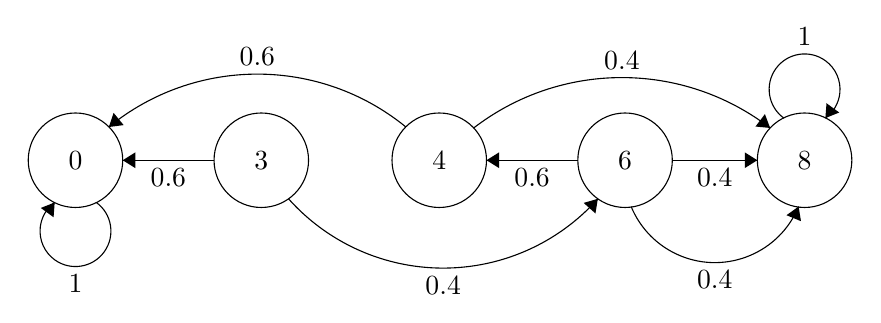
\begin{tikzpicture}[scale=0.2]
\tikzstyle{every node}+=[inner sep=0pt]
\draw [black] (13.6,-32.1) circle (3);
\draw (13.6,-32.1) node {$0$};
\draw [black] (25.4,-32.1) circle (3);
\draw (25.4,-32.1) node {$3$};
\draw [black] (36.7,-32.1) circle (3);
\draw (36.7,-32.1) node {$4$};
\draw [black] (48.5,-32.1) circle (3);
\draw (48.5,-32.1) node {$6$};
\draw [black] (59.9,-32.1) circle (3);
\draw (59.9,-32.1) node {$8$};
\draw [black] (14.923,-34.78) arc (54:-234:2.25);
\draw (13.6,-39.35) node [below] {$1$};
\fill [black] (12.28,-34.78) -- (11.4,-35.13) -- (12.21,-35.72);
\draw [black] (22.4,-32.1) -- (16.6,-32.1);
\fill [black] (16.6,-32.1) -- (17.4,-32.6) -- (17.4,-31.6);
\draw (19.5,-32.6) node [below] {$0.6$};
\draw [black] (15.721,-29.985) arc (129.16845:50.83155:14.929);
\fill [black] (15.72,-29.99) -- (16.66,-29.87) -- (16.02,-29.09);
\draw (25.15,-26.13) node [above] {$0.6$};
\draw [black] (46.775,-34.546) arc (-41.72198:-138.27802:13.163);
\fill [black] (46.77,-34.55) -- (45.87,-34.81) -- (46.62,-35.48);
\draw (36.95,-39.45) node [below] {$0.4$};
\draw [black] (45.5,-32.1) -- (39.7,-32.1);
\fill [black] (39.7,-32.1) -- (40.5,-32.6) -- (40.5,-31.6);
\draw (42.6,-32.6) node [below] {$0.6$};
\draw [black] (59.516,-35.041) arc (-22.38587:-157.61413:5.749);
\fill [black] (59.52,-35.04) -- (58.75,-35.59) -- (59.67,-35.97);
\draw (54.2,-39.1) node [below] {$0.4$};
\draw [black] (38.886,-30.052) arc (127.56838:52.43162:15.44);
\fill [black] (57.71,-30.05) -- (57.38,-29.17) -- (56.78,-29.96);
\draw (48.3,-26.35) node [above] {$0.4$};
\draw [black] (51.5,-32.1) -- (56.9,-32.1);
\fill [black] (56.9,-32.1) -- (56.1,-31.6) -- (56.1,-32.6);
\draw (54.2,-32.6) node [below] {$0.4$};
\draw [black] (58.577,-29.42) arc (234:-54:2.25);
\draw (59.9,-24.85) node [above] {$1$};
\fill [black] (61.22,-29.42) -- (62.1,-29.07) -- (61.29,-28.48);
\end{tikzpicture}
\end{center}
and the equations are:

\begin{align*}
\phi(3) &= 0.4\phi(6) \\
\phi(6) &= 0.4 \phi(8) + 0.6\phi(4) \\
\phi(4) &= 0.4 \phi(8) \\
\phi(0) &= 0 \\
\phi(8) &= 1
\end{align*}
We solve and find 
\begin{equation*}
\phi(3) = 0.256, \phi(4) = 0.4, \phi(6) = 0.64
\end{equation*}
\end{solution}

\item
Which strategy gives Smith the better chance of getting out of jail?
\begin{solution}[0.5cm]
By comparing the third components of the vector $\phi$ we find that 
the bold strategy gives Smith a better chance to get our of jail.
\end{solution}
\end{enumerate}